\chapter{Einleitung}

\section{Einführung und Motivation}

Die BRUNATA-METRONA GmbH \& Co. KG zählt seit mehr als 50 Jahren zu den führenden Anbietern verbrauchsbasierter Abrechnungssysteme für Heiz- und Wasserkosten. Das Unternehmen hat seine Marktposition durch die schrittweise Erweiterung seines Dienstleistungsangebots und den gezielten Einsatz digitaler Tools gesichert. Diese strategische Ausrichtung half dabei, auch in komplexen Phasen der Branchenentwicklung wettbewerbsfähig zu bleiben.

Um die Effizienz weiter zu steigern und Dienstleistern bzw. Kunden neue Interaktionsmöglichkeiten zu bieten, evaluieren Abteilungen regelmäßig neue Technologien für die Integration in bestehende Abläufe. Hier stehen aktuell vor allem KI-gestützte Lösungen, wie die Implementierung eines Chatbots zur Unterstützung der Kundenkommunikation, und die Verwendung von Computer Vision Algorithmen für die automatisierte Ablesung von Zählerständen im Fokus.

Letzteres stellt die Grundlage der Augmented Reality (AR) Technologie dar, die in den letzten Jahren zunehmend an Bedeutung gewonnen hat. AR ermöglicht die Einblendung digitaler Informationen in die reale Welt und eröffnet damit vielfältige Anwendungsmöglichkeiten. Diese Technologie hat in den letzten Jahren eine rasante Entwicklung durchlaufen und rückte somit sowohl bei BRUNATA-METRONA als auch branchenübergreifend in den Fokus. Treiber dieser Entwicklung sind verbesserte Hard- und Software-Austattung bei mobilen Smart-Geräten, praxistaugliche Smartglasses sowie Fortschritte in KI-gestützter Bilderkennung und -verarbeitung. Diese Fortschritte in der Computer Vision machen AR zunehmend alltagstauglich und interessant für diverse Einsatzgebiete.

Im Folgenden soll die Technologie von AR hinsichtlich der theoretischen Grundlagen, technischen Implementierungsmöglichkeiten und dem Potenzial zur Optimierung von Geschäftsprozessen untersucht werden.

\section{Augmented Reality}

Augmented Reality (AR) ist eine Technologie, die die reale Welt durch die Einbindung digitaler Informationen und virtueller Objekte erweitert und dabei gegebenenfalls Interaktionen zwischen Nutzern und diesen digitalen Elementen ermöglicht. Im Gegensatz zu Virtual Reality (VR), die Benutzer vollständig in eine künstliche Umgebung eintauchen lässt, bewahrt AR die Sicht auf die reale Welt. Dadurch wird die Realität ergänzt, statt sie zu ersetzen. (\cite{azuma1997ar})

Die Ursprünge von AR reichen bis in die 1960er Jahre zurück, als Ivan Sutherland mit seiner Vision des 'ultimativen Displays' (\citet{sutherland1965ultimateDisplay}) den Grundstein legte. In seinen Forschungen philosophierte Sutherland über die Möglichkeit einer interaktiven, computergenerierten Welt, die er als '[...] ein Wunderland, wie Alice es betrat' beschrieb. Im Jahr 1968 entwickelte er gemeinsam mit seinem Studenten Bob Sproull ein Head-Mounted-Display, das es Nutzern erstmals ermöglichte, einfache dreidimensionale Formen in der realen Umgebung zu visualisieren. Dazu trägt der Benutzer eine Art Smartglasses auf dem Kopf die an der Decke befestigt sind. Das Gerät zeichnet die Rotation des Kopfes auf und überträgt die Bewegungen auf die virtuellen Objekte, die durch die Linsen sichtbar werden. Dies gilt als die erste praktische Anwendung von AR. (\cite{sutherland19683dDisplay, doerner2022virtual})

\begin{figure}
    \centering
    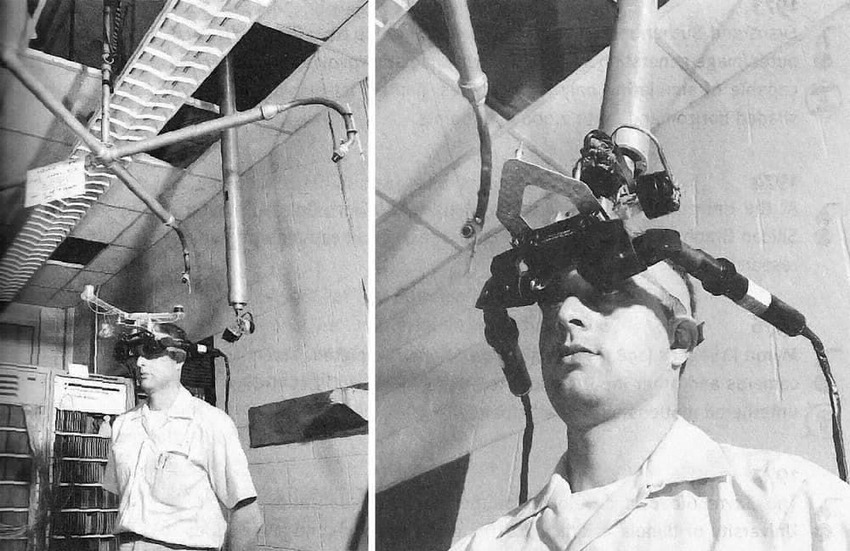
\includegraphics[ width=.5\textwidth ]{HeadMountedDisplay}
    \caption{Sutherland's Head Mounted Display\label{fig:HeadMountedDisplay}}\par
\end{figure}

In den darauffolgenden Jahrzehnten wurden zahlreiche technologische Hürden überwunden, die die Entwicklung von AR zuvor behindert hatten. Fortschritte bei der Rechenleistung, die Miniaturisierung von Sensoren sowie die kontinuierliche Verbesserung der Bildverarbeitung ebneten den Weg für den heutigen Erfolg von AR-Anwendungen. (\cite{doerner2022virtual})

Die neuartigen Möglichkeiten, Informationen auf visuell ansprechende und interaktive Weise darzustellen, eröffnen ein breites Spektrum an Einsatzgebieten. Dieses Potenzial wurde in verschiedenen Branchen erkannt und in innovativen Anwendungen umgesetzt. Ein populäres Beispiel ist das mobile Spiel 'Pokémon Go' aus dem Jahr 2016, bei dem Spieler virtuelle Monster in der realen Welt fangen. In der Medizin dient AR der Visualisierung medizinischer Daten und der Unterstützung bei chirurgischen Eingriffen, wodurch Präzision und Behandlungsergebnisse verbessert werden können. Zuletzt lösten Meta und Apple mit ihren AR-Brillen Meta 2 und Apple Glass eine neue Welle der Begeisterung für AR aus und brachten die Technologie in den Fokus der Öffentlichkeit. (\cite{doerner2022virtual, boulanger2024applications})

\section{Zielsetzung}

Ziel dieser Arbeit ist es, das Potenzial von Augmented Reality zur Optimierung von Geschäftsprozessen in einem praxisnahen Anwendungsszenario aufzuzeigen. Bei diesem Szenario handelt es sich um die Montage von Rauchmeldern, einem alltäglichen Prozess in der BRUNATA-METRONA GmbH \& Co. KG.

Dazu sollen die theoretischen Grundlagen von AR hinsichtlich der Implementierung einer Anwendung für  mobile Endgeräte untersucht und zusammengefasst werden. Dabei werden mathematische Konzepte und Algorithmen, die für die Umsetzung von AR-Anwendungen relevant sind, erläutert und anhand von Beispielen verdeutlicht. 

Im Rahmen dieser Untersuchung soll ein Prototyp einer mobilen AR-Anwendung entworfen und umgesetzt werden, welche den Prozess der Montage von Rauchmeldern visuell unterstützt. Dabei sollen die Vorteile von AR genutzt werden, um den Prozess effizienter und benutzerfreundlicher zu gestalten. Der entwickelte Prototyp wird in einer praxisnahen Umgebung getestet und evaluiert, um die Effektivität der AR-Technologie zu bewerten und mögliche Optimierungspotenziale zu identifizieren.

Darüber hinaus wird das Potenzial von AR für den Einsatz in produktiven Umgebungen kritisch reflektiert. Dabei werden die Integration der Technologie in bestehende Prozesse sowie ihre langfristigen Auswirkungen diskutiert.

Die Ergebnisse dieser Arbeit sollen als Entscheidungsgrundlage für die Einführung von AR-Technologien im Montageprozess von Rauchmeldern und als Grundlage für zukünftige AR-Projekte bei der BRUNATA-METRONA dienen.

\section{Struktur der Arbeit}

TODO

